\documentclass[../Main.tex]{subfiles}

\begin{document}
\author{Diffraction} %use author for title of lesson
\date{Year 1 Topic 18} %use date to refer to topic in main booklet

\section{Diffraction} %Section is the title of the lesson repeated, ready for the main contents page.

\begin{frame}{Diffraction}
    Not to be confused with refraction, diffraction is where waves spread out when interacting with an obstacle. This obstacle could be a gap to pass through, or an object in the path of, the wave. 
    
    \begin{figure}
        \centering
        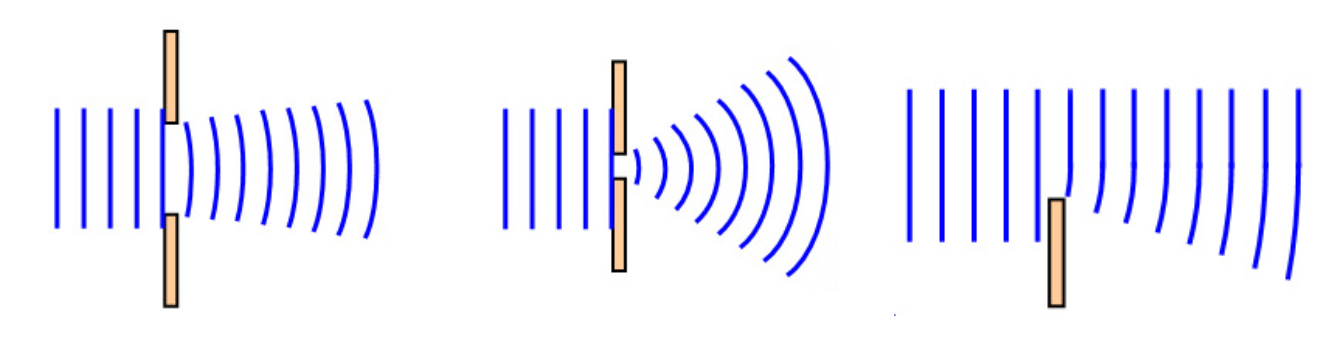
\includegraphics[width=\textwidth]{Waves_Images/diffraction.png}
    \end{figure}
    \pause
    \begin{block}{Diffraction}
    Diffraction does not change the wavespeed, frequency, or wavelength of a wave. It simply spreads out the wave. 
    \end{block}
\end{frame}

\begin{frame}{Diffraction}
    The closer a gap is the wavelength of the wave, the more diffraction occurs -- but if the gap is smaller than the wavelength, it is completely blocked. \pause
    \newline
    Similar is true for an obstacle, the closer the obstacle is to the wavelength the more it will diffract, but any larger and it will mostly block the wave.
    
    \begin{figure}
        \centering
        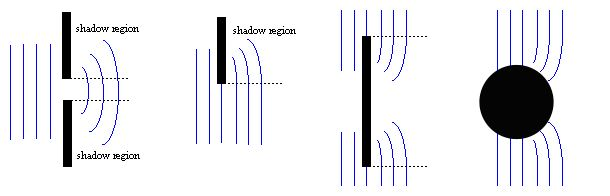
\includegraphics[width=\textwidth]{Waves_Images/shadowregion.png}
    \end{figure}
\end{frame}

\begin{frame}{Diffraction of light}
    When light passes through a single slit, it will diffract through the slit, producing a pattern on a screen. It is observed that there are bright and dark fringes of light. 
    
    \begin{figure}
    \begin{subfigure}
        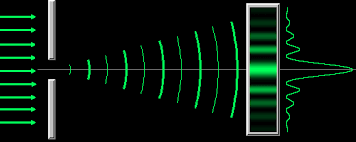
\includegraphics[height=2.5cm]{Waves_Images/greenlaser_singleslit.png}
    \end{subfigure}
        \begin{subfigure}
            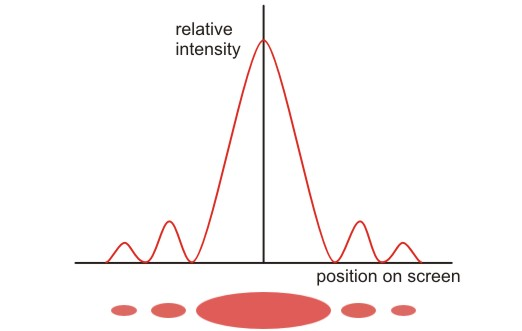
\includegraphics[height=2.5cm]{Waves_Images/diffractionintensitygraph.jpg}
        \end{subfigure}
    \end{figure}
    
    If asked to sketch a single-slit diffraction pattern, you will be required to show the relative intensity of the central maxima to be much higher than the others and the width to be double of the other fringes.
\end{frame}

\begin{frame}{Diffraction of white light}
    The amount of diffraction depends on the wavelength of light -- for the same slit, red light will diffract more as the slit is smaller compared to the wavelength.
    \begin{figure}
        \centering
        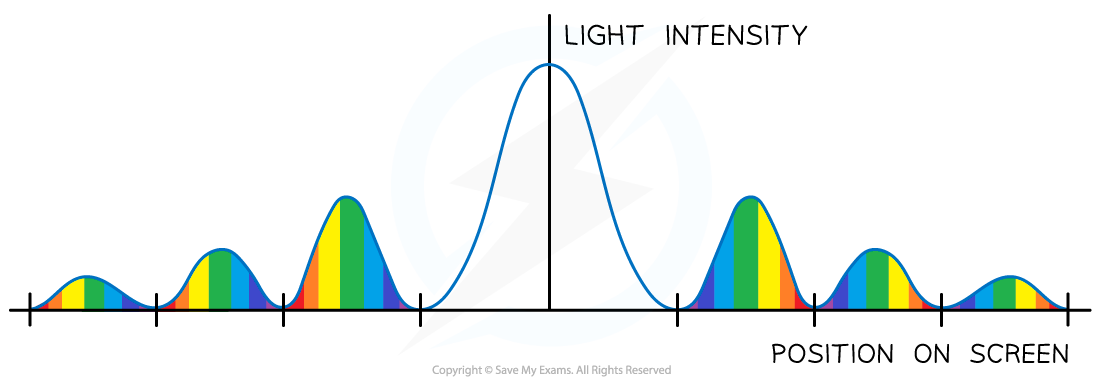
\includegraphics[width=\textwidth]{Waves_Images/White-Light-Diffraction.png}
    \end{figure}
    This has the effect of rainbow fringes, but with a central bright white fringe where blue is closer to the center on each fringe
\end{frame}

\begin{frame}{Young's Double Slit}
\begin{multicols}{2}
    In the 1800s Thomas Young performed an experiment that created an interference pattern from sunlight, where wave fronts are parallel to each other. 
    \newline
    
    He set up a single slit to create a single circular wave front which fed into a double slit. The double slit now had two sources of coherent light, which would be otherwise impossible with the technology available at the time. This then produced an interference pattern on a screen, similar to the sound interference patterns we saw previously.
    \columnbreak
    \begin{figure}
        \centering
        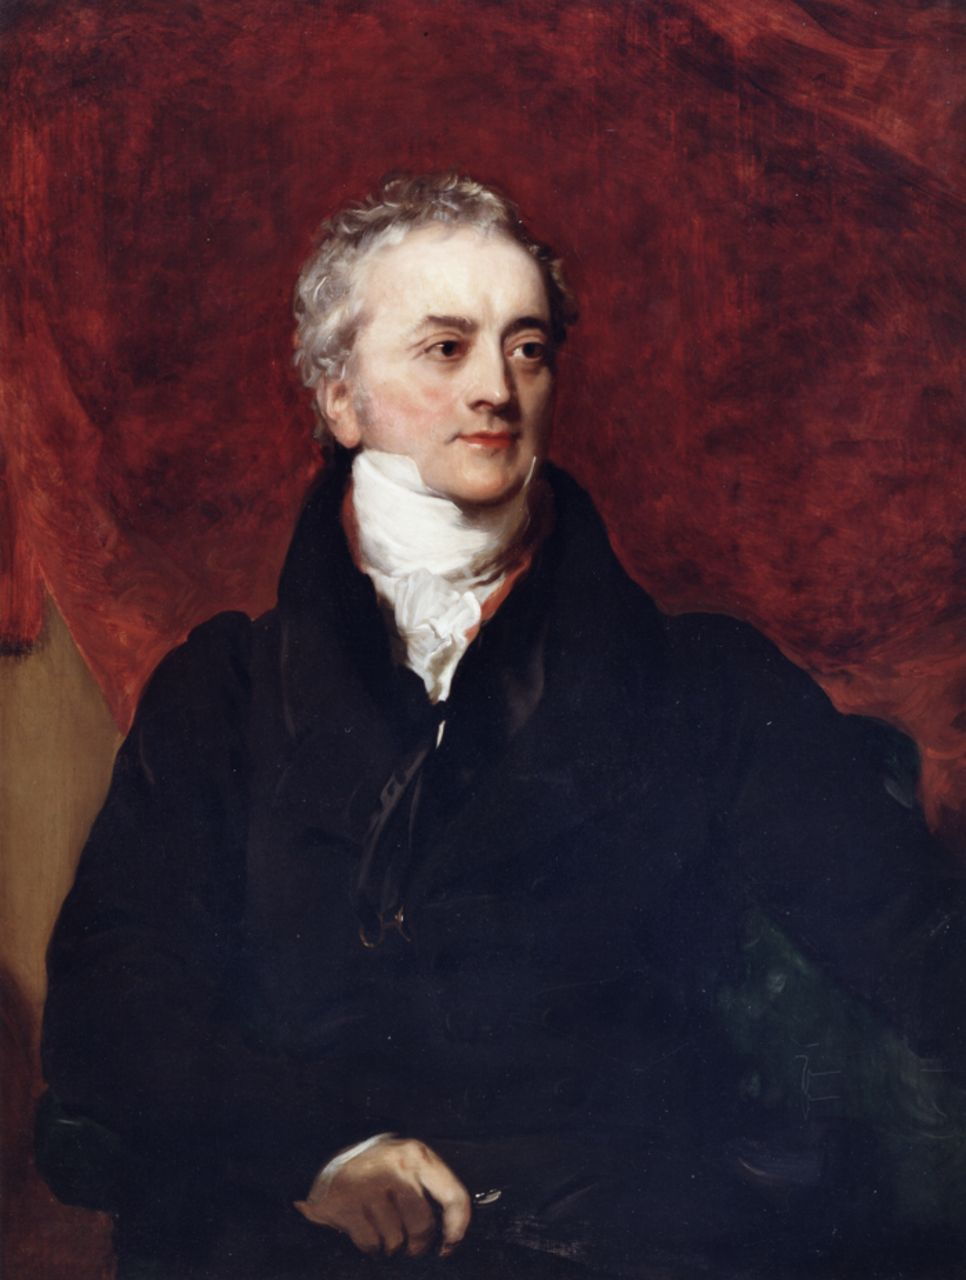
\includegraphics[height=5cm]{Waves_Images/thomasyoung.png}
    \end{figure}
   A diagram of the experiment set-up is on the next slide! You must be able to sketch this!
\end{multicols}
\end{frame}

\begin{frame}{Young's Double Slit}
Note that Young also created monochromatic light for use by including a colour filter before the single slit.
     \begin{figure}
        \centering
        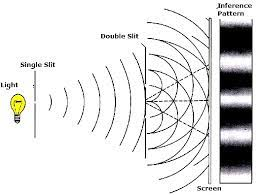
\includegraphics[height=5cm]{Waves_Images/doubleslit.png}
    \end{figure}
    --What variables might affect the pattern observed?
\end{frame}

\begin{frame}{Young's Double Slit}
    \begin{itemize}
        \item D - the distance from double slits to screen. Unit: meters
        \item a - the slit separation (from center to center). Unit: meters
        \item $\lambda$ - the wavelength of light. Unit: meters
    \end{itemize}
    Using these we can determine the separation between adjacent maxima (or minima):
    \pause
    \begin{equation*}
        x=\frac{\lambda D}{a}
    \end{equation*} or as given on your formula sheet it is rearranged for $\lambda$ as the experiment is usually used to determine an unknown wavelength.
    
    \begin{alertblock}{Double slit only!}
This equation can only be used for a double slit!! 
    \end{alertblock}
    We can work with double slits using a laser - removing the need for a single slit as a laser produces coherent light by default. 
\end{frame}

\begin{frame}{Examples}
    \begin{exampleblock}{Example 1}
    Monochromatic light of wavelength 600nm is directed at two parallel narrow slits spaced at 0.1mm
apart. The transmitted light falls on a screen 1.8m from the slits. Calculate the fringe spacing. \pause
--10cm
    \end{exampleblock} \pause
    
    \begin{exampleblock}{Example 2}
    In a double slit experiment, a screen is positioned at a distance of 0.80m from two slits. Light of wavelength 590nm is directed at the slits to give an interference pattern on the screen with two fringes 4.8mm apart. Calculate the slit spacing. %\paue
    -- $98\mu m$
    \end{exampleblock}
\end{frame}

\end{document}